\chapter{Models} \label{sec:model}

\section{XY model on self-avoiding walks (SAWs)} \label{sec:xymodel}

A molecular conformation of the length $N$ is represented by a self-avoiding walk (SAW) on a regular lattice with $N-1$ edges and $N$ nodes.  Each $i$th node represents a spin-like variable $s_i$ which is associated with angle $\theta_i \in  [-\pi;\pi]$. Figure \ref{fig:example} illustrates the model on the square lattice. 

 \begin{figure}[H]
	\centering
	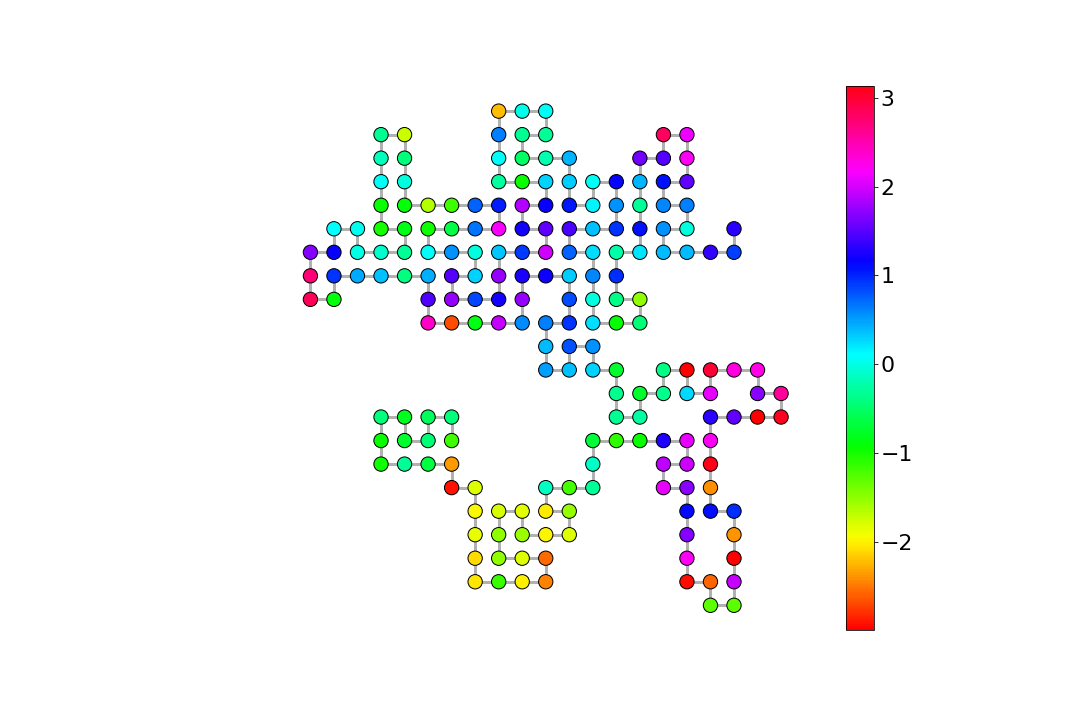
\includegraphics[scale=0.20]{Images/state_example.png}
	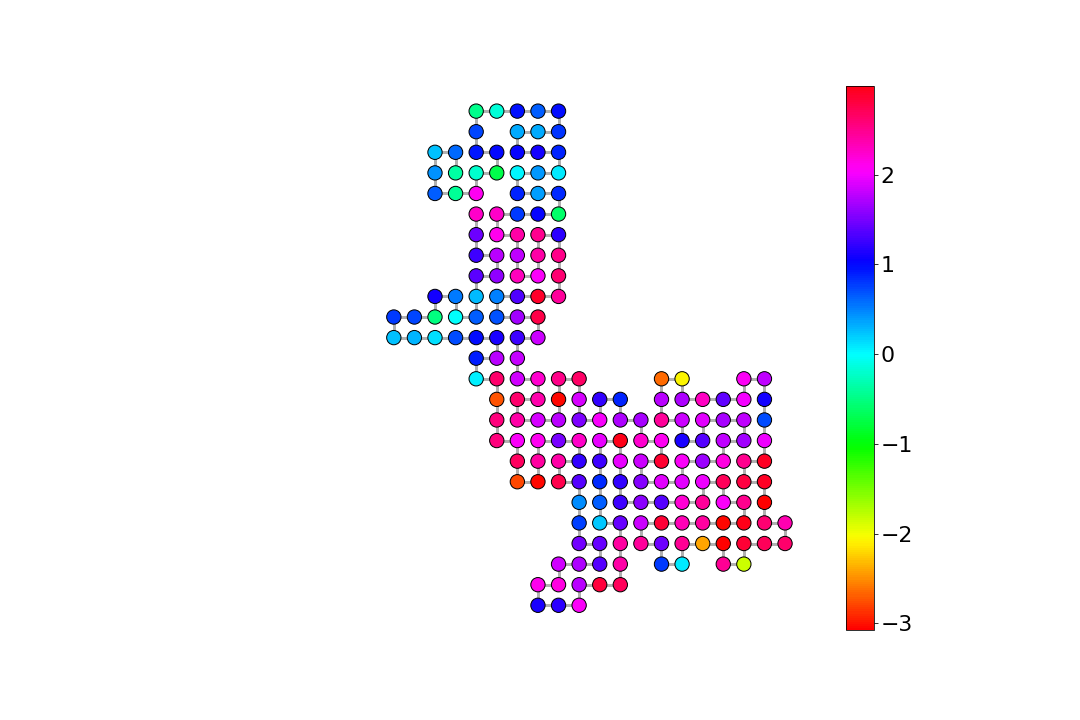
\includegraphics[scale=0.20]{Images/state_example1.png}
	%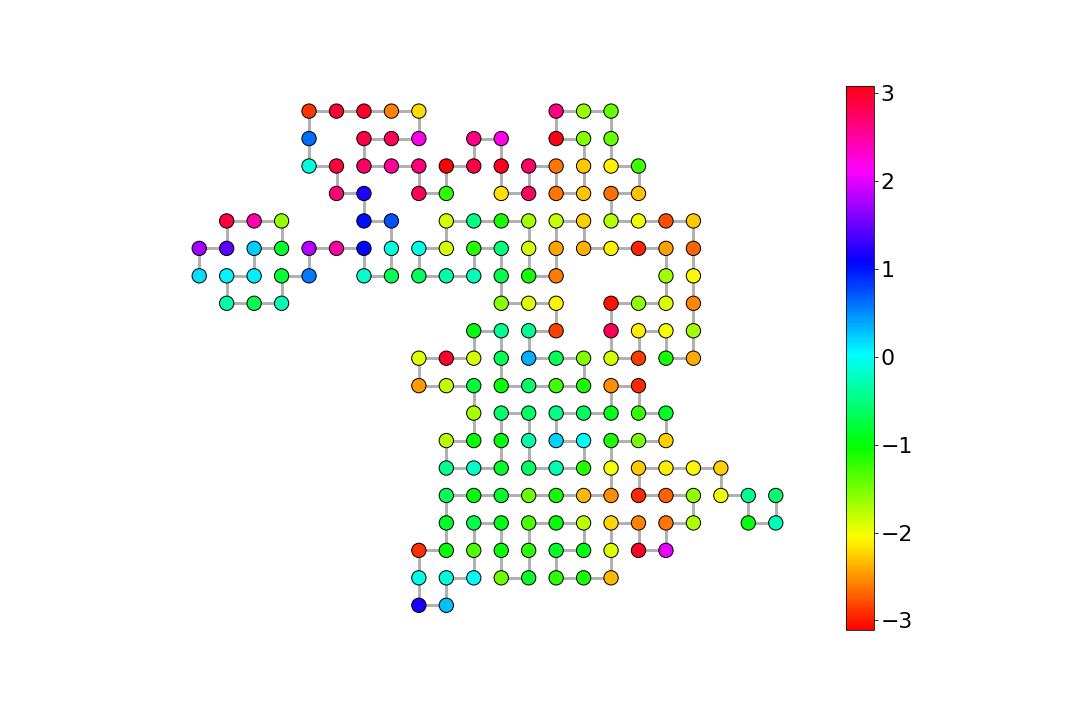
\includegraphics[scale=0.18]{Images/state_example2.png}
	\caption{ Example states of the  chain $N=200$ obtained using simulation at $J=1.41$ on the square lattice. The color represents angle variable $\theta_i$. }
	\label{fig:example}
\end{figure}


 The Hamiltonian for sequence of spins $s$ and conformation $u$ is defined as the sum over all  non-repeating neighbor  pairs $\langle i, j \rangle$th in conformation:
\begin{equation}
\label{hamiltonian}
H(u,s) = -J \sum_{ \langle i, j \rangle } cos(\theta_i - \theta_j) - h \sum_i cos(\theta_i)
\end{equation}

In our work, we focus on the system in lack of an external field: $h=0$.  
Without loss of generality, we assume that $\beta = \frac{1}{kT} = 1$, where $k$ is Boltzmann’s constant, $T$ is temperature. 

Let $U_N$ be a set of all SAW conformations of N monomers. The partition function for the chain of the length $N$ is the sum over all SAW conformations of N monomers and the integral over all spin space:  
\begin{equation}
\label{partitionfunction}
Z(J) =  \sum_{u \in U_N }  \int_{-\pi}^{\pi}   \frac{1}{ (2 \pi  )^N}
     d \theta_1 d \theta_2 \dots d\theta_N
 e ^{J \cos(\theta_1-\theta_2)} e ^{J \cos(\theta_2-\theta_3)} \dots 
 e ^{J \cos(\theta_{N-1}-\theta_N)} %= 2 \pi
 %\prod_{j=2}^{N}  \int_{-\pi}^{\pi} d \theta_j^{'} e ^{J(cos\theta_j^{'})} 
\end{equation}

The mean magnetization is defined as a vector:
\begin{equation}
\label{meanmagnetization}
\langle \vec{m} \rangle = \frac{1}{N} \left\langle ( \sum_{i=1}^{N} cos \theta_i, \sum_{i=1}^{N} sin \theta_i  ) \right\rangle
\end{equation}

The second moment of magnetization is a square of the norm:
\begin{equation}
\label{secondmomentmagnetization}
\langle m^2 \rangle = \frac{1}{N^2} \left\langle ( \sum_{i=1}^{N} cos \theta_i )^2 +  (\sum_{i=1}^{N} sin \theta_i  )^2 \right\rangle
\end{equation}

From measurements of the average magnetization per spin $\langle m \rangle (J)$, we can obtain the value of the magnetic cumulant  (Binder parameters) of fourth order \cite{Binder2010}, which is helpful to study magnetic phase transition:
\begin{equation}
\label{binderqum}
U_4 (J) = 1 - \frac{ \langle m^4 \rangle}{3 \langle m^2 \rangle^2  }
\end{equation}

The Binder parameter  could be used to determine the order of magnetic parameters \cite{binder1981finite}.  At some
continuous phase transition, the Binder ratio transitions approaches a step function as the system size is increased. The Binder ratio  has a divergent feature at the step if the system has the first order transition. 

\subsection{Case without interaction (J=0)} \label{U4J0}

Consider the case when no interaction which could be close to classical 1-dimensional XY-chain. In case of open boundary conditions, the partition function for the chain of the length $N$ has following form:  
\begin{equation}
\label{partitionfunction_free}
Z(J) =    \int_{-\pi}^{\pi} \frac{1}{ (2 \pi  )^N}       d \theta_1 d \theta_2 \dots d\theta_N
e ^{Jcos(\theta_1-\theta_2)} e ^{Jcos(\theta_2-\theta_3)} \dots 
e ^{Jcos(\theta_{N-1}-\theta_N)} %= 2 \pi
%\prod_{j=2}^{N}  \int_{-\pi}^{\pi} d \theta_j^{'} e ^{J(cos\theta_j^{'})} 
\end{equation}

In case $J=0$ (high-temperature regime), all states have equal probabilities:
\begin{equation}
\label{paritionfunction_free_zero}
Z(0) =  %\prod_{j=1}^{N}  
\int_{-\pi}^{\pi} (\frac{1}{2 \pi})^N   d \theta_1 d \theta_2 \dots d\theta_N 
 %d \theta_j^{'} 
\end{equation}
To calculate the exact value of $\langle m^2 \rangle (J=0)$  we use following results: 
\begin{equation*} 
 \int_{-\pi}^{\pi}  \frac{1}{2 \pi} sin^2 \theta d \theta =\int_{-\pi}^{\pi}  \frac{1}{2 \pi} cos^2 \theta d \theta = \frac{1}{2} 
\end{equation*}
 \begin{equation*} \int_{-\pi}^{\pi}  \frac{1}{2 \pi} sin \theta d \theta  =\int_{-\pi}^{\pi}  \frac{1}{2 \pi} cos  \theta d \theta = 0 \end{equation*}
   After some calculation, only integration results for $N$ times $sin^2 \theta_i$ and $N$ times $cos^2 \theta_i$ survive:
\begin{equation} 
\label{m2j0}
  \langle m^2 \rangle (J=0) = \frac{1}{N^2}   \int_{-\pi}^{\pi}  (\frac{1}{2 \pi})^N \left(  
   ( \sum_{i=1}^{N} cos \theta_i )^2 +  (\sum_{i=1}^{N} sin \theta_i  )^2 \right)  d \theta_1 d \theta_2 \dots d\theta_N =
  \frac{1}{N^2}  (\frac{1}{2}N +\frac{1}{2}N)   = \frac{1}{N}
\end{equation}
Next, to calculate $\langle m^4 \rangle (J=0)$ we use following facts: 
\begin{equation*}
\langle m^4 \rangle (J=0) = \frac{1}{N^4}   \int_{-\pi}^{\pi}  (\frac{1}{2 \pi})^N \left(  
( \sum_{i=1}^{N} cos \theta_i )^2 +  (\sum_{i=1}^{N} sin \theta_i  )^2 \right)^2 d \theta_1 d \theta_2 \dots d\theta_N  
\end{equation*} \\ 
\begin{equation*}
 \left(  
( \sum_{i=1}^{N} cos \theta_i )^2 +  (\sum_{i=1}^{N} sin \theta_i  )^2 \right)^2 =  (\sum_{i=1}^{N} cos \theta_i )^4 + (\sum_{i=1}^{N} sin \theta_i )^4 + 2 ( \sum_{i=1}^{N} cos \theta_i )^2( \sum_{i=1}^{N} sin \theta_i )^2 
\end{equation*} \\

$ \int_{-\pi}^{\pi}  \frac{1}{2 \pi} sin^4 \theta d \theta =\int_{-\pi}^{\pi}  \frac{1}{2 \pi} cos^4 \theta d \theta = \frac{3}{8}$ (We  have $N$ times $sin^4\theta_i$-term and $N$ times $cos^4\theta_i$-term  what results in $2\times \frac{3}{8} \times N$). \\

$ \int_{-\pi}^{\pi}  \frac{1}{2 \pi}\int_{-\pi}^{\pi} \frac{1}{2 \pi} sin^2 \theta_i sin^2 \theta_j d\theta_i  d\theta_j = \int_{-\pi}^{\pi}  \frac{1}{2 \pi}\int_{-\pi}^{\pi} \frac{1}{2 \pi} cos^2 \theta_i cos^2 \theta_j d\theta_i  d\theta_j = \frac{1}{4}$ (We  have $6N(N-1)\frac{1}{2}$ times $sin$-term and $6N(N-1)\frac{1}{2}$ times $cos$-term  what results in $6\times \frac{1}{4} \times N(N-1)$). \\

$ \int_{-\pi}^{\pi}  \frac{1}{2 \pi} sin^2 \theta cos^2 \theta d \theta  = \frac{1}{8}$ (We  have this term $2N$ times  what results in $2\times \frac{1}{8} \times N$). \\

$ \int_{-\pi}^{\pi}  \frac{1}{2 \pi}\int_{-\pi}^{\pi} \frac{1}{2 \pi} cos^2 \theta_i sin^2 \theta_j d\theta_i  d\theta_j = \frac{1}{4}$ (We  have $2N(N-1)\frac{1}{2}$ times  what results in $2\times \frac{1}{4} \times N(N-1)$). \\

All other terms with odd power of sin of cos function equals zero after integration over period. 
\begin{equation*}
\langle m^4 \rangle (J=0) = \frac{1}{N^4} \left( 2\times \frac{3}{8} \times N + 6\times \frac{1}{4} \times N(N-1) + 2\times \frac{1}{8} \times N + 2\times \frac{1}{4} \times N(N-1)
\right) = \frac{2N-1}{N^3}  
\end{equation*}
\begin{equation}
\label{binderqum_0}
U_4 (J=0) = 1 - \frac{  \frac{2N-1}{N^3} }{3  \frac{1}{N^2} } = 1 - 
\frac{2N-1}{3N} = \frac{1}{3} + \frac{1}{3N} 
\end{equation}
 
 In classical Ising model, $U_4 \rightarrow 0$ as $J \rightarrow 0$. In our work, we use the common definition for Binder cumulant. Consequently, the lower limiting value in disordered state is $U_4 = \frac{1}{3}$.
 
\section{Structural properties} 
To study structural phase transition, we use the mean square end-to-end distance (radius) of self-avoiding-walks which is defined as the sum over all configurations:
\begin{equation}
\label{endtoend}
\langle R_N^2 \rangle  =  \frac{1}{Z_N} \sum_{ |u|=N }  |u|^2 e^{-H(s,u)},
\end{equation}
where $|u|$ is the Euclidean distance between the endpoints of conformation $u$, and $Z_N$ is partition function in the canonical assemble \eqref{partitionfunction_free}. We call it "mean radius" for brevity. As $N \rightarrow \infty $, the mean radius  of SAWs is believed to scale as 
\begin{equation}
\label{r_scale}
\langle R_N^2 \rangle \sim N^{2 \nu }.
\end{equation}
Here ${\nu} $ is a critical exponent, which is model-dependent.   For thermodynamic limit $N \rightarrow \infty $, $\nu$ is believed to have the form of a step function of interaction energy $J$. For finite systems, this effect is rounded \cite{vanderzande1998lattice}. 

We define the scaling function for two chain lengths $N_1$, $N_2$:

\begin{equation*}
\label{r1r2}
\langle R_{N_1}^2 \rangle \sim N_1^{2 \nu }; \langle R_{N_2}^2 \rangle \sim N_2^{2 \nu }
\end{equation*}

\begin{equation*}
\label{logr1r2}
\log  \left(  \frac{ \langle R_{N_1}^2 \rangle}  {\langle R_{N_2}^2 \rangle}  \right) \sim  2\nu \log  \left(  \frac{ N_1}  {N_2}  \right)
\end{equation*}

\begin{equation}
\label{varphir}
 \varphi_{R^2} =  \frac{   \log  \left(  \frac{ \langle R_{N_1}^2 \rangle}  {\langle R_{N_2}^2 \rangle}  \right) }{ \log  \left(  \frac{ N_1}  {N_2}  \right) }
\end{equation}
For large $N \rightarrow$, the crossing point of curves $\varphi_{R^2}$ is expected to predict structural phase transition point. 

At low $J < J_{\theta}$, the system is equivalent to SAW without interaction. One should call to mind the classical homopolymer model which is represented by an interacting, or collapsing, self-avoiding walk (iSAW). Below we briefly report known critical values for homopolymer which are important in our work as iSAW is a parental model of XY on SAWs. 


\subsection{SAW on a 2D square lattice }
%Consider collapsing self-avoiding walks, or classical homopolymer model (see chapter 9 in Ref.\cite{van2015statistical}. For thermodynamic limit $N \rightarrow \infty $, $\nu$ is believed to have the form of a step function of interaction energy $J$. For finite systems, this effect is rounded \cite{vanderzande1998lattice}. At low $J < J_{\theta}$, the system is equivalent to SAW without interaction. 
Focus on collapsing self-avoiding walks, or classical homopolymer model (see chapter 9 in Ref.\cite{van2015statistical}. At $J=0$, spins become irrelevant and XY model on SAWs  is equivalent to non-interacting SAWs.  The exact value of critical  exponent for non-interacting SAWs ($J=0$)\cite{Li1995}
\begin{equation}
\label{nur}
\nu = \frac{3}{4}. 
\end{equation}
At the theta-point, $\nu_{\theta}$  is obtained via Coulomb-gas approximations \cite{Duplantier1987}:
\begin{equation}
\label{nu_theta}
\nu_{\theta} = \frac{4}{7}.
\end{equation}  
For the globular regime ($J > J_{\theta}$) in 2D case:
\begin{equation}
\label{globular}
\nu = \frac{1}{d} = \frac{1}{2}.
\end{equation} 

\subsection{SAW on a 3D cubic lattice }

For 3D case, Flory predicted value for non-interacting self-avoiding walk as follows \cite{flory1953principles}:
\begin{equation}
\label{eq:nu_3D_J0_flory}
 \nu = \frac{3}{2+d} = \frac{3}{5}.
\end{equation}
The critical exponent $\nu$ was also estimated numerically \cite{Li1995}:
\begin{equation}
\label{eq:nu_3D_J0_sokal}
\nu = 0.5877 \pm 0.0006.
\end{equation}
 At the theta-point, the $\nu_{\theta}$  is \cite{van2015statistical} 
 \begin{equation}
 \label{eq:nu_3D_Jtheta_flory}
 \nu = \frac{1}{2}.
 \end{equation}
 For compact regime when $J > J_{\theta}$, the critical exponent $\nu$  has following value:  
\begin{equation}
\label{eq:nu_3D_Jglobular_flory}
\nu = \frac{1}{d} = \frac{1}{3}.
\end{equation}
% $\int_{-\pi}^{\pi}  \frac{1}{2 \pi} sin \theta =\int_{-\pi}^{\pi}  \frac{1}{2 \pi} cos  \theta  = 0 $. 
%\begin{equation*}
% \langle m^2 \rangle (J=0) = \frac{1}{N^2} 
%  2 \pi \prod_{j=2}^{N}  \int_{-\pi}^{\pi} sin^2  \theta_j+ cos^2 \theta_j  d \theta_j^{'} = 2 \pi \left[  \int_{-\pi}^{\pi} sin^2  \theta_j+ cos^2 \theta_j  d \theta_j^{'}  \right]^{N-1} = 2 \times 2^{N-1} \pi ^N  
%\end{equation*}
%\begin{equation*}
%\langle m^4 \rangle (J=0) = \frac{1}{N^4} 
%2 \pi \prod_{j=2}^{N}  \int_{-\pi}^{\pi} (sin^2  \theta_j+ cos^2 \theta_j)^2 d \theta_j^{'} = 2 \pi \left[  \int_{-\pi}^{\pi} (sin^2  \theta_j+ cos^2 \theta_j )^2 d \theta_j^{'}  \right]^{N-1} = 2 \times 2^{N-1} \pi ^N
%\end{equation*}
%\begin{equation*}
% \langle ( \sum_{i=1}^{N} cos \theta_i )^2  \rangle = 
%2 \pi \prod_{j=2}^{N}  \int_{-\pi}^{\pi} cos^2 \theta_j d \theta_j^{'} = 2 \pi  \left[ \int_{-\pi}^{\pi} cos^2 \theta_j d \theta_j^{'} \right] ^{N-1} = 2 \pi ^{N}
%\end{equation*}
%\begin{equation*}
%\langle ( \sum_{i=1}^{N} sin \theta_i )^2  \rangle = 
%2 \pi \prod_{j=2}^{N}  \int_{-\pi}^{\pi} sin^2 \theta_j d \theta_j^{'} = 2 \pi  \left[ \int_{-\pi}^{\pi} sin^2 \theta_j d \theta_j^{'} \right] ^{N-1} = 2 \pi ^{N}
%\end{equation*}
%\begin{equation*}
% \langle m^2 \rangle (J=0) = \frac{1}{N^2} \langle ( \sum_{i=1}^{N} cos \theta_i )^2 +  (\sum_{i=1}^{N} sin \theta_i  )^2 \rangle =  \frac{1}{N^2} 2 \pi ^{N} +  \frac{1}{N^2} 2 \pi ^{N} = \frac{1}{N^2} 4 \pi ^N
%\end{equation*}
%\begin{equation*}
% \langle m^4 \rangle = 2 \pi \prod_{j=2}^{N}  \int_{-\pi}^{\pi} sin^2 \theta_j d \theta_j^{'} 
%\end{equation*}
%\begin{equation*}
% \langle m^4 \rangle = \langle (m^2)^2 \rangle = \left\langle  
% \left( \frac{1}{N^2}   ( \sum_{i=1}^{N} cos \theta_i )^2 + \frac{1}{N^2}  (\sum_{i=1}^{N} sin \theta_i  )^2 \right)^2 
% \right\rangle = \frac{4}{N^4} 2^{2N} \pi ^{2N}
%\end{equation*}
